
\chapter{神经网络——深度学习的核心}

\intro{本章是全书的枢纽章节。我们将从感知机出发，逐层揭示多层神经网络的数学原理：前向传播如何逐层变换表示，反向传播如何高效计算梯度，以及激活函数、损失函数、正则化等技术如何共同塑造现代深度学习。你将分别用NumPy和PyTorch亲手实现一个能识别手写数字的多分类神经网络。}

%%%%%%%%%%%%%%%%%%%%%%%%%%%%%%%%%%%%%%%%%%%%%%%%%%%%%%%%
\section{从感知机到多层神经网络}

\subsection{神经元——最基本的计算单元}

神经网络的基本组成单元是\textbf{人工神经元}（artificial neuron）。它接收一组输入信号，加权求和后经激活函数变换输出：

\[
z = \sum_{i=1}^{n} w_i x_i + b = \mathbf{w}^{\top}\mathbf{x} + b, \qquad a = g(z)
\]

其中 $\mathbf{w} \in \R^{n}$ 为权重向量，$b$ 为偏置，$g(\cdot)$ 为激活函数。

\begin{figure}[H]\centering
\begin{tikzpicture}[
    mynode/.style={circle, draw=blue!60, thick, fill=blue!10, minimum size=1.2cm},
    myinput/.style={circle, draw=green!60!black, thick, fill=green!10, minimum size=0.9cm},
    myarrow/.style={->, >=stealth, thick},
]
\node[mynode] (n1) at (0,2.5) {$x_1$};
\node[mynode] (n2) at (0,1.0) {$x_2$};
\node[mynode] (n3) at (0,-0.5) {$x_3$};
\node (dots) at (0,-2.0) {$\vdots$};
\node[mynode] (nn) at (0,-3.5) {$x_n$};

\node[mynode, draw=red!60, fill=red!10] (sum) at (4,-0.5) {$\Sigma$};
\node[mynode, draw=orange!60, fill=orange!10] (act) at (7,-0.5) {$g(\cdot)$};

\draw[myarrow] (n1.east) -- node[above, font=\footnotesize] {$w_1$} (sum.west);
\draw[myarrow] (n2.east) -- node[above, font=\footnotesize] {$w_2$} (sum.west);
\draw[myarrow] (n3.east) -- node[above, font=\footnotesize] {$w_3$} (sum.west);
\draw[myarrow] (nn.east) -- node[above, font=\footnotesize] {$w_n$} (sum.west);
\draw[myarrow] (sum.east) -- node[above, font=\footnotesize] {$z$} (act.west);
\draw[myarrow] (act.east) -- ++(1.2,0) node[right] {$a = g(z)$};

\node[font=\footnotesize, below=0.3cm of sum] {加权求和};
\node[font=\footnotesize, below=0.3cm of act] {激活输出};

\node[font=\footnotesize] at (1.5,-4.5) {$b$（偏置）};
\draw[myarrow, dashed, gray] (3.5,-4.5) -- (sum.south);
\end{tikzpicture}
\caption{人工神经元的结构。输入信号 $x_1,\dots,x_n$ 经权重 $w_i$ 加权求和后加偏置 $b$，再经激活函数 $g(\cdot)$ 变换产生输出 $a$}
\label{fig:single-neuron}
\end{figure}

模型参数中，\textbf{权重} $w_i$ 表示输入 $x_i$ 对输出的影响程度，\textbf{偏置} $b$ 允许神经元在没有输入时也有非零输出——相当于线性模型中的截距项。

单个神经元等价于线性模型（若 $g$ 为恒等映射）或广义线性模型。单神经元的表达能力有限，只能解决线性可分问题。

\subsection{单层网络与异或问题}

将多个神经元并排放置，构成\textbf{单层神经网络}（也称单隐藏层）：

\[
\mathbf{a}^{[1]} = g(\mathbf{W}^{[1]}\mathbf{x} + \mathbf{b}^{[1]}), \qquad
\hat{\mathbf{y}} = \mathbf{W}^{[2]}\mathbf{a}^{[1]} + \mathbf{b}^{[2]}
\]

其中 $\mathbf{W}^{[1]} \in \R^{h \times n_x}$ 为第一层权重（$h$ 个神经元，每个 $n_x$ 维输入），$\mathbf{W}^{[2]} \in \R^{n_y \times h}$ 为输出层权重。

单隐藏层的网络已经具备\textbf{万能逼近}能力——只要有足够多的隐藏神经元，它可以逼近任意连续函数。然而，单层网络无法高效解决XOR（异或）问题：XOR是非线性可分的，需要至少两层隐藏层才能用紧致的分段线性边界成功分类。

\begin{figure}[H]\centering
\begin{tikzpicture}[scale=1.2]
\fill[blue!10] (0,0) circle (3pt) node[above right, font=\tiny] {$(0,0)=0$};
\fill[red!10] (2,0) circle (3pt) node[above right, font=\tiny] {$(1,0)=1$};
\fill[red!10] (0,2) circle (3pt) node[above right, font=\tiny] {$(0,1)=1$};
\fill[blue!10] (2,2) circle (3pt) node[above right, font=\tiny] {$(1,1)=0$};

\draw[->] (-0.5,0) -- (2.8,0) node[right] {$x_1$};
\draw[->] (0,-0.5) -- (0,2.8) node[above] {$x_2$};

\draw[dashed, red!70, thick] (-0.2,1.2) -- (2.2,1.1);
\draw[dashed, red!70, thick] (1.1,-0.2) -- (1.2,2.2);
\node[font=\footnotesize] at (2.5,-0.8) {单条直线无法分离};
\end{tikzpicture}
\caption{XOR问题的几何直观。蓝色点输出0，红色点输出1。单条直线（单层感知机）无法分开这两类点}
\label{fig:xor-problem}
\end{figure}

\subsection{多层网络与表示学习}

\textbf{多层神经网络}通过堆叠多个隐藏层，逐层提取越来越抽象的特征表示：

\[
\mathbf{a}^{[l]} = g(\mathbf{W}^{[l]}\mathbf{a}^{[l-1]} + \mathbf{b}^{[l]}), \quad l = 1, 2, \dots, L
\]

\begin{figure}[H]\centering
\begin{tikzpicture}[
    mynode/.style={circle, draw=blue!60, thick, fill=blue!10, minimum size=0.8cm, inner sep=0pt},
    myarrow/.style={->, >=stealth, thick, gray!60},
]
% Input layer
\foreach \i in {1,...,4} {
    \node[mynode, fill=green!10, draw=green!60!black] (in\i) at (0, 3.5-1.2*\i) {};
}
% Hidden 1
\foreach \i in {1,...,5} {
    \node[mynode] (h1\i) at (3, 4.0-1.0*\i) {};
}
% Hidden 2
\foreach \i in {1,...,5} {
    \node[mynode] (h2\i) at (6, 4.0-1.0*\i) {};
}
% Hidden 3
\foreach \i in {1,...,4} {
    \node[mynode] (h3\i) at (9, 3.5-1.2*\i) {};
}
% Output
\foreach \i in {1,2} {
    \node[mynode, fill=red!10, draw=red!60] (out\i) at (12, 2.0-1.5*\i) {};
}

% Connections (simplified)
\foreach \i in {1,...,4} {
    \foreach \j in {1,...,5} {
        \draw[myarrow, opacity=0.3] (in\i) -- (h1\j);
    }
}
\foreach \i in {1,...,5} {
    \foreach \j in {1,...,5} {
        \draw[myarrow, opacity=0.3] (h1\i) -- (h2\j);
    }
}
\foreach \i in {1,...,5} {
    \foreach \j in {1,...,4} {
        \draw[myarrow, opacity=0.3] (h2\i) -- (h3\j);
    }
}
\foreach \i in {1,...,4} {
    \foreach \j in {1,2} {
        \draw[myarrow, opacity=0.3] (h3\i) -- (out\j);
    }
}

\node[font=\footnotesize] at (0,4.5) {输入层};
\node[font=\footnotesize] at (3,5.0) {隐藏层1};
\node[font=\footnotesize] at (6,5.0) {隐藏层2};
\node[font=\footnotesize] at (9,5.0) {隐藏层3};
\node[font=\footnotesize] at (12,2.8) {输出层};

\node[font=\small\bfseries] at (6,-1.5) {深度 = 层数 $L$，宽度 = 每层神经元数量};
\end{tikzpicture}
\caption{具有三个隐藏层的深度神经网络。浅层学习简单的局部特征，深层将这些特征组合为更复杂的抽象表示}
\label{fig:deep-network}
\end{figure}

深度学习的核心优势在于\textbf{层次化表示学习}：
\begin{itemize}
    \item 浅层神经元学习\textbf{低级特征}（边缘、纹理、音调）
    \item 中层神经元将低级特征\textbf{组合}为中级特征（形状、部件、音素）
    \item 深层神经元构建\textbf{高级语义}概念（物体、人脸、词语含义）
\end{itemize}

%%%%%%%%%%%%%%%%%%%%%%%%%%%%%%%%%%%%%%%%%%%%%%%%%%%%%%%%
\section{激活函数——神经网络的灵魂}

没有激活函数，多层网络等价于单层线性模型——线性变换的复合仍然是线性变换。激活函数引入\textbf{非线性}，赋予网络表达能力。

\subsection{Sigmoid 与 Tanh}

早期神经网络中最常用的两种激活函数：

\begin{myformula}
\begin{aligned}
\sigma(z) &= \frac{1}{1 + e^{-z}}, \quad \sigma(z) \in (0, 1) \\[4pt]
\sigma'(z) &= \sigma(z)(1 - \sigma(z))
\end{aligned}
\end{myformula}

\[
\tanh(z) = \frac{e^{z} - e^{-z}}{e^{z} + e^{-z}}, \quad \tanh(z) \in (-1, 1), \quad \tanh'(z) = 1 - \tanh^2(z)
\]

\begin{figure}[H]\centering
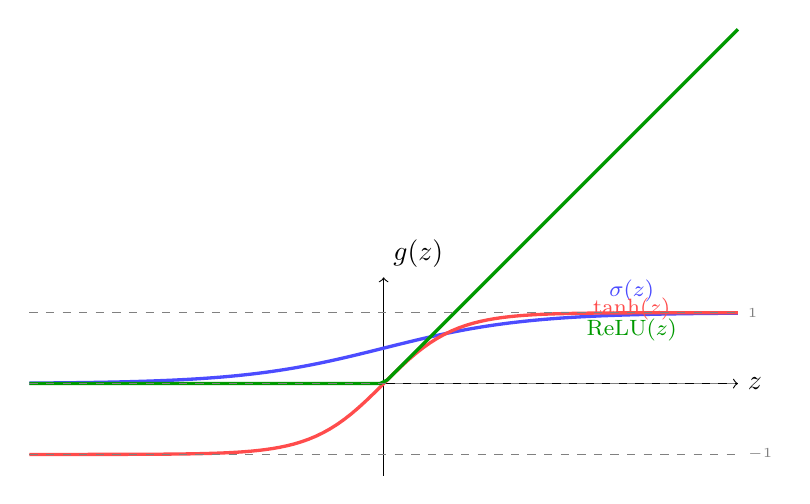
\begin{tikzpicture}[scale=0.9]
\draw[->] (-5,0) -- (5,0) node[right] {$z$};
\draw[->] (0,-1.3) -- (0,1.5) node[above] {};
\node[above right] at (0,1.5) {$g(z)$};

\draw[blue!70, very thick, domain=-5:5, samples=100] plot (\x, {1/(1+exp(-\x))});
\node[blue!70, font=\footnotesize] at (3.5,1.3) {$\sigma(z)$};

\draw[red!70, very thick, domain=-5:5, samples=100] plot (\x, {(exp(\x)-exp(-\x))/(exp(\x)+exp(-\x))});
\node[red!70, font=\footnotesize] at (3.5,1.05) {$\tanh(z)$};

\draw[green!60!black, very thick, domain=-5:5, samples=100] plot (\x, {max(0,\x)});
\node[green!60!black, font=\footnotesize] at (3.5,0.75) {ReLU$(z)$};

\draw[dashed, gray] (-5,0) -- (5,0);
\draw[dashed, gray] (-5,1) -- (5,1) node[right, font=\tiny] {$1$};
\draw[dashed, gray] (-5,-1) -- (5,-1) node[right, font=\tiny] {$-1$};
\end{tikzpicture}
\caption{三种常见激活函数的曲线对比。Sigmoid将输出压缩到$(0,1)$，Tanh压缩到$(-1,1)$，ReLU在正半轴保持线性}
\label{fig:activation-functions}
\end{figure}

\subsection{ReLU 及其变体}

\textbf{ReLU}（Rectified Linear Unit）是现代神经网络中使用最广泛的激活函数：

\[
\text{ReLU}(z) = \max(0, z), \quad \text{ReLU}'(z) = \begin{cases} 1 & z > 0 \\ 0 & z < 0 \end{cases}
\]

ReLU的优点：解决梯度消失问题（正半区导数为1）、计算高效（只需比较和取max）、具有稀疏激活特性（负半区输出为0）。

ReLU的缺点：``死亡ReLU''问题——如果大梯度导致权重更新使得某个神经元对所有输入都输出负值，该神经元的梯度恒为0，永远无法恢复。

\textbf{Leaky ReLU} 解决死亡神经元问题：

\[
\text{LeakyReLU}(z) = \max(\alpha z, z), \quad \alpha \text{ 通常取 } 0.01
\]

\textbf{GELU}（Gaussian Error Linear Unit）是BERT和GPT中使用的激活函数，将ReLU的硬阈值平滑化：

\[
\text{GELU}(z) = z \cdot \Phi(z) \approx z \cdot \sigma(1.702z)
\]

其中 $\Phi(z)$ 是标准正态分布的累积分布函数。GELU的平滑性使其在Transformer架构中表现优于ReLU。

\subsection{Softmax——多分类的输出层}

对于 $K$ 类分类问题，\textbf{Softmax} 函数将原始得分（logits）映射为概率分布：

\[
\text{softmax}(\mathbf{z})_i = \frac{e^{z_i}}{\sum_{j=1}^{K} e^{z_j}}, \quad i=1,\dots,K
\]

Softmax的性质：输出非负且和为1；保持输入的大小顺序（单调性）；对平移不敏感：$\text{softmax}(\mathbf{z} + c) = \text{softmax}(\mathbf{z})$。

\begin{mycode}{激活函数的PyTorch实现对比}
\begin{lstlisting}[language=Python]
import torch
import torch.nn as nn
import torch.nn.functional as F
import matplotlib.pyplot as plt

z = torch.linspace(-5, 5, 1000)

activations = {
    'Sigmoid':   F.sigmoid(z),
    'Tanh':      F.tanh(z),
    'ReLU':      F.relu(z),
    'LeakyReLU': F.leaky_relu(z, negative_slope=0.01),
    'GELU':      F.gelu(z),
    'Softplus':  F.softplus(z),       # 平滑版ReLU: log(1+e^z)
    'Swish':     z * F.sigmoid(z),    # 自门控激活
}

fig, axes = plt.subplots(2, 4, figsize=(14, 7))
for ax, (name, y) in zip(axes.flat, activations.items()):
    ax.plot(z.numpy(), y.numpy(), 'b-', lw=2)
    ax.set_title(name); ax.grid(True, alpha=0.3)
    ax.set_xlabel('z'); ax.set_ylabel('g(z)')

# 在PyTorch中作为层使用
relu_layer = nn.ReLU()
gelu_layer = nn.GELU()
leaky_layer = nn.LeakyReLU(0.01)
\end{lstlisting}
\end{mycode}

%%%%%%%%%%%%%%%%%%%%%%%%%%%%%%%%%%%%%%%%%%%%%%%%%%%%%%%%
\section{前向传播——信息的流动}

\subsection{前向传播的矩阵形式}

给定一个 $L$ 层网络，前向传播将输入 $\mathbf{x} \in \R^{n_x}$ 逐层变换为最终输出 $\hat{\mathbf{y}}$：

\begin{myformula}
\begin{aligned}
\mathbf{z}^{[1]} &= \mathbf{W}^{[1]}\mathbf{x} + \mathbf{b}^{[1]}, \quad
\mathbf{a}^{[1]} = g^{[1]}(\mathbf{z}^{[1]}) \\
\mathbf{z}^{[2]} &= \mathbf{W}^{[2]}\mathbf{a}^{[1]} + \mathbf{b}^{[2]}, \quad
\mathbf{a}^{[2]} = g^{[2]}(\mathbf{z}^{[2]}) \\
&\;\;\vdots \\
\mathbf{z}^{[L]} &= \mathbf{W}^{[L]}\mathbf{a}^{[L-1]} + \mathbf{b}^{[L]}, \quad
\hat{\mathbf{y}} = \mathbf{a}^{[L]} = g^{[L]}(\mathbf{z}^{[L]})
\end{aligned}
\end{myformula}

其中 $\mathbf{W}^{[l]} \in \R^{n_l \times n_{l-1}}$，$\mathbf{b}^{[l]} \in \R^{n_l}$，$\mathbf{a}^{[l]} \in \R^{n_l}$。

在前向传播中，网络从数据中提取特征的过程可以理解为逐层的\textbf{坐标变换}：每一层将前一层输出的特征空间进行线性变换（旋转、缩放、投影）后再经非线性扭曲，逐步构造出最适合当前任务的特征表示。

\subsection{向量化——批量前向传播}

在训练和推理中，我们通常一次处理多个样本（mini-batch）。将 $m$ 个样本堆叠为矩阵 $\mathbf{X} \in \R^{n_x \times m}$，前向传播的向量化形式为：

\[
\mathbf{Z}^{[1]} = \mathbf{W}^{[1]}\mathbf{X} + \mathbf{b}^{[1]}, \quad
\mathbf{A}^{[1]} = g^{[1]}(\mathbf{Z}^{[1]})
\]

其中 $\mathbf{b}^{[1]}$ 通过\textbf{广播}（broadcasting）加到每一列。这种向量化写法利用底层BLAS库的优化矩阵乘法，比显式的for循环快数十到数百倍。

%%%%%%%%%%%%%%%%%%%%%%%%%%%%%%%%%%%%%%%%%%%%%%%%%%%%%%%%
\section{损失函数——定义优化目标}

\subsection{均方误差（MSE）}

回归问题最常用的损失函数：

\[
\mathcal{L}_{\text{MSE}} = \frac{1}{m}\sum_{i=1}^{m} \|\hat{\mathbf{y}}^{(i)} - \mathbf{y}^{(i)}\|_2^2
\]

MSE对异常值敏感（平方放大大误差），但在高斯噪声假设下等价于最大似然估计。

\subsection{交叉熵损失}

分类问题的标准选择。对于二分类（$y \in \{0, 1\}$）：

\[
\mathcal{L}_{\text{BCE}} = -\frac{1}{m}\sum_{i=1}^{m}\left[y^{(i)}\log\hat{y}^{(i)} + (1-y^{(i)})\log(1-\hat{y}^{(i)})\right]
\]

对于多分类（$K$类），使用分类交叉熵：

\[
\mathcal{L}_{\text{CE}} = -\frac{1}{m}\sum_{i=1}^{m}\sum_{k=1}^{K} y_k^{(i)}\log\hat{y}_k^{(i)}
\]

其中 $\mathbf{y}^{(i)}$ 是one-hot向量，$\hat{\mathbf{y}}^{(i)}$ 是Softmax输出的概率分布。

交叉熵来自信息论：$H(p, q) = -\sum_x p(x)\log q(x)$ 衡量真实分布 $p$ 与预测分布 $q$ 之间的差异。最小化交叉熵等价于最大化正确类别的对数似然。交叉熵配合Softmax在反向传播时具有优美的梯度形式：

\[
\frac{\partial \mathcal{L}_{\text{CE}}}{\partial z_k} = \hat{y}_k - y_k
\]

这一简洁的梯度形式是交叉熵损失被广泛使用的重要原因。

\begin{mycode}{常见损失函数的PyTorch实现}
\begin{lstlisting}[language=Python]
import torch
import torch.nn as nn

# MSE (回归)
mse_loss = nn.MSELoss()
y_pred = torch.randn(32, 1)
y_true = torch.randn(32, 1)
loss_mse = mse_loss(y_pred, y_true)

# 二分类交叉熵 (BCEWithLogits包含Sigmoid，数值更稳定)
bce_loss = nn.BCEWithLogitsLoss()
logits = torch.randn(32, 1)       # 原始得分，未经Sigmoid
labels = torch.randint(0, 2, (32, 1)).float()
loss_bce = bce_loss(logits, labels)

# 多分类交叉熵 (CrossEntropyLoss包含Softmax)
ce_loss = nn.CrossEntropyLoss()
logits = torch.randn(32, 10)      # 原始得分，(batch, classes)
labels = torch.randint(0, 10, (32,))
loss_ce = ce_loss(logits, labels)

# 手动计算（理解原理）
def cross_entropy_manual(logits, labels, n_classes=10):
    probs = torch.softmax(logits, dim=1)
    labels_onehot = torch.zeros_like(logits)
    labels_onehot.scatter_(1, labels.unsqueeze(1), 1)
    return -(labels_onehot * torch.log(probs + 1e-9)).sum(dim=1).mean()

loss_manual = cross_entropy_manual(logits, labels)
print(f"PyTorch: {loss_ce.item():.6f}")
print(f"Manual:  {loss_manual.item():.6f}")
print(f"Match:   {torch.allclose(loss_ce, loss_manual, atol=1e-5)}")
\end{lstlisting}
\end{mycode}

%%%%%%%%%%%%%%%%%%%%%%%%%%%%%%%%%%%%%%%%%%%%%%%%%%%%%%%%
\section{反向传播——学习的引擎}

\subsection{链式法则}

反向传播（Backpropagation）是计算梯度的核心算法。它基于微积分的链式法则：对于复合函数 $f(g(x))$，有

\[
\frac{df}{dx} = \frac{df}{dg} \cdot \frac{dg}{dx}
\]

在神经网络中，损失 $\mathcal{L}$ 是参数 $\{\mathbf{W}^{[l]}, \mathbf{b}^{[l]}\}_{l=1}^{L}$ 的复合函数。链式法则允许我们从输出层开始，逐层反向计算梯度：

\[
\frac{\partial\mathcal{L}}{\partial\mathbf{W}^{[l]}} = \frac{\partial\mathcal{L}}{\partial\mathbf{z}^{[l]}} \cdot \frac{\partial\mathbf{z}^{[l]}}{\partial\mathbf{W}^{[l]}}
\]

\subsection{反向传播的逐步推导}

考虑一个 $L$ 层网络（第 $l$ 层激活函数为 $g^{[l]}$），损失函数为 $\mathcal{L}(\hat{\mathbf{y}}, \mathbf{y})$。反向传播从输出层开始：

\textbf{步骤1：初始化}。计算输出层的误差：
\[
\delta^{[L]} = \frac{\partial\mathcal{L}}{\partial\mathbf{z}^{[L]}} = \frac{\partial\mathcal{L}}{\partial\mathbf{a}^{[L]}} \odot g^{[L]\prime}(\mathbf{z}^{[L]})
\]

对于Softmax + 交叉熵的组合，$\delta^{[L]} = \hat{\mathbf{y}} - \mathbf{y}$。

\textbf{步骤2：反向迭代}。对于 $l = L-1, L-2, \dots, 1$：
\[
\delta^{[l]} = \left(\mathbf{W}^{[l+1]\top}\delta^{[l+1]}\right) \odot g^{[l]\prime}(\mathbf{z}^{[l]})
\]

\textbf{步骤3：计算梯度}：
\[
\frac{\partial\mathcal{L}}{\partial\mathbf{W}^{[l]}} = \delta^{[l]}\mathbf{a}^{[l-1]\top}, \qquad
\frac{\partial\mathcal{L}}{\partial\mathbf{b}^{[l]}} = \delta^{[l]}
\]

\textbf{步骤4：参数更新}。使用梯度下降更新：
\[
\mathbf{W}^{[l]} \leftarrow \mathbf{W}^{[l]} - \eta\,\frac{\partial\mathcal{L}}{\partial\mathbf{W}^{[l]}}, \qquad
\mathbf{b}^{[l]} \leftarrow \mathbf{b}^{[l]} - \eta\,\frac{\partial\mathcal{L}}{\partial\mathbf{b}^{[l]}}
\]

\subsection{反向传播的计算复杂度}

反向传播的巧妙之处在于：它通过复用中间计算结果，使得梯度计算的时间复杂度与前向传播\textbf{相同}（都是 $O(\sum_{l} n_l n_{l-1})$），而非简单地对每个参数独立计算梯度那样的 $O((\sum n_l)^2)$。这是深度学习得以扩展到亿万级别参数的内在原因。

\begin{myTheorem}{反向传播的计算效率}
对于一个 $L$ 层的全连接网络，前向传播和反向传播的计算复杂度均正比于网络中所有突触连接的数量。这一性质使得训练极深网络在计算上是可行的。
\end{myTheorem}

\begin{figure}[H]\centering
\begin{tikzpicture}[
    mynode/.style={rectangle, draw=blue!60, thick, fill=blue!5, minimum width=2.2cm, minimum height=0.7cm, font=\footnotesize, rounded corners=2pt},
    myarrow/.style={->, >=stealth, thick, blue!60},
    mygrad/.style={->, >=stealth, thick, dashed, red!60},
]
\node[mynode] (l1) {$\mathbf{z}^{[1]}, \mathbf{a}^{[1]}$};
\node[mynode] (l2) [below=1.2cm of l1] {$\mathbf{z}^{[2]}, \mathbf{a}^{[2]}$};
\node[mynode] (l3) [below=1.2cm of l2] {$\mathbf{z}^{[3]}, \mathbf{a}^{[3]}$};
\node[mynode] (loss) [below=1.2cm of l3] {$\mathcal{L}(\hat{\mathbf{y}}, \mathbf{y})$};

\draw[myarrow] (l1) -- (l2) node[midway, right, font=\tiny] {前向};
\draw[myarrow] (l2) -- (l3) node[midway, right, font=\tiny] {前向};
\draw[myarrow] (l3) -- (loss) node[midway, right, font=\tiny] {前向};

\draw[mygrad] (loss) -- (l3) node[midway, left, font=\tiny, red!70!black] {$\delta^{[3]}$};
\draw[mygrad] (l3) -- (l2) node[midway, left, font=\tiny, red!70!black] {$\delta^{[2]}$};
\draw[mygrad] (l2) -- (l1) node[midway, left, font=\tiny, red!70!black] {$\delta^{[1]}$};

\node[font=\small\bfseries, blue!60] at (4.5,1.5) {前向传播};
\node[font=\small\bfseries, red!60] at (4.5,1.0) {反向传播};
\end{tikzpicture}
\caption{前向传播存储中间激活值，反向传播利用这些缓存值计算各层参数的梯度}
\label{fig:backprop-flow}
\end{figure}

\subsection{局部误差的直观解释}

反向传播中的 $\delta_j^{[l]}$ 表示改变第 $l$ 层的第 $j$ 个神经元的线性输出 $z_j^{[l]}$ 对最终损失的影响程度。它可以拆解为两个因子的乘积：

\[
\delta_j^{[l]} = \underbrace{\left(\sum_{k} W_{kj}^{[l+1]} \delta_k^{[l+1]}\right)}_{\text{来自第 $l+1$ 层的反馈}} \times \underbrace{g^{[l]\prime}(z_j^{[l]})}_{\text{本层激活函数的梯度}}
\]

这个形式揭示了反向传播的本质：每个神经元通过与后一层神经元的连接权重，接收来自后层的``误差反馈''，再乘以自身激活函数的导数，得到本层输出的误差信号。

%%%%%%%%%%%%%%%%%%%%%%%%%%%%%%%%%%%%%%%%%%%%%%%%%%%%%%%%
\section{梯度消失与梯度爆炸}

\subsection{问题成因}

深度网络训练中的核心困难。以Sigmoid激活函数为例，$\sigma'(z) = \sigma(z)(1-\sigma(z))$ 在 $z$ 较大或较小时的导数趋近于0。在反向传播中，梯度需要逐层乘以激活函数的导数：

\[
\frac{\partial\mathcal{L}}{\partial\mathbf{W}^{[1]}} = \delta^{[1]}\mathbf{x}^{\top}, \quad
\delta^{[1]} = \mathbf{W}^{[2]\top}\sigma'(\mathbf{z}^{[2]})\odot\mathbf{W}^{[3]\top}\sigma'(\mathbf{z}^{[3]})\odot\cdots
\]

经过多层的连乘，梯度呈\textbf{指数级衰减}（梯度消失）或\textbf{指数级增长}（梯度爆炸）。

\begin{mydefinition}{梯度消失与梯度爆炸}
如果 $\forall l, \|\mathbf{W}^{[l]}\| \cdot \|g^{[l]\prime}\| < 1$，梯度在反向传播中指数衰减，早期层的参数几乎停止更新。反之，如果乘积远大于1，梯度指数增长，参数更新量极大，训练发散。
\end{mydefinition}

\subsection{解决方案}

\begin{itemize}
    \item \textbf{ReLU激活函数}：正半区梯度恒为1，根本解决Sigmoid/Tanh的饱和问题
    \item \textbf{权重初始化}：Xavier初始化（保持前向和反向方差稳定）、He初始化（适配ReLU）
    \item \textbf{Batch Normalization}：将每层输入的分布标准化，使激活值落在激活函数的非饱和区
    \item \textbf{残差连接}（ResNet）：提供梯度的``高速公路''，使梯度可以直接流到浅层
    \item \textbf{梯度裁剪}：限制梯度的范数，防止梯度爆炸
\end{itemize}

%%%%%%%%%%%%%%%%%%%%%%%%%%%%%%%%%%%%%%%%%%%%%%%%%%%%%%%%
\section{正则化——防止过拟合}

\subsection{$L^1$ 与 $L^2$ 正则化}

在损失函数中加入参数范数的惩罚项，限制模型复杂度：

\[
\mathcal{L}_{\text{reg}} = \mathcal{L}(\hat{\mathbf{y}}, \mathbf{y}) + \frac{\lambda}{2}\|\mathbf{W}\|_2^2 \quad (L^2 \text{ 正则化，Ridge，梯度衰减})
\]

\[
\mathcal{L}_{\text{reg}} = \mathcal{L}(\hat{\mathbf{y}}, \mathbf{y}) + \lambda\|\mathbf{W}\|_1 \quad (L^1 \text{ 正则化，Lasso，稀疏化})
\]

$L^2$ 正则化（权重衰减）：所有权重向零方向收缩，防止任何单个权重过大。$L^1$ 正则化：产生稀疏解，自动特征选择。

\subsection{Dropout}

\textbf{Dropout} 是深度神经网络中最高效的正则化技术之一。在训练时，每个神经元以概率 $p$（通常 $p=0.5$）被随机丢弃：

\[
a_j^{[l]} = \begin{cases} 0 & \text{以概率 } p \\ a_j^{[l]} / (1-p) & \text{以概率 } 1-p \end{cases}
\]

除以 $1-p$（inverted dropout）使得训练时的期望激活值不变，推理时无需任何缩放。

Dropout 的直观解释：相当于训练大量子网络的集成。每次迭代随机丢弃不同神经元，迫使网络学习冗余的、鲁棒的表示，而非依赖某个特定神经元的输出。

\begin{mycode}{Dropout 在 PyTorch 中的应用}
\begin{lstlisting}[language=Python]
import torch.nn as nn

class MLPWithDropout(nn.Module):
    def __init__(self, in_dim, hidden_dim, out_dim, dropout_p=0.5):
        super().__init__()
        self.net = nn.Sequential(
            nn.Linear(in_dim, hidden_dim),
            nn.ReLU(),
            nn.Dropout(p=dropout_p),          # 训练时随机丢�?        nn.Linear(hidden_dim, hidden_dim),
            nn.ReLU(),
            nn.Dropout(p=dropout_p),
            nn.Linear(hidden_dim, out_dim)
        )

    def forward(self, x):
        return self.net(x)

model = MLPWithDropout(784, 256, 10, dropout_p=0.3)

# 训练模式：Dropout 生效
model.train()
out_train = model(torch.randn(4, 784))  # 每次前向，不同神经元被丢�?
# 评估模式：Dropout 关闭（所有神经元参与，无缩�?
model.eval()
out_eval = model(torch.randn(4, 784))
\end{lstlisting}
\end{mycode}

\subsection{Batch Normalization 的正则化效应}

BN除了加速训练，还有轻微的正则化效果：mini-batch的均值和方差作为噪声源，类似于Dropout的随机扰动。不过这种正则化效果很弱，通常不能单独替代Dropout或权重衰减。

%%%%%%%%%%%%%%%%%%%%%%%%%%%%%%%%%%%%%%%%%%%%%%%%%%%%%%%%
\section{用NumPy从零实现神经网络}

为深入理解神经网络的本质，我们用纯NumPy实现一个用于MNIST二分类（数字0 vs 非0）的两层网络。

\begin{mycode}{NumPy 实现的完整两层神经网络}
\begin{lstlisting}[language=Python]
import numpy as np

def sigmoid(z):
    return 1 / (1 + np.exp(-z))

def relu(z):
    return np.maximum(0, z)

def initialize_parameters(n_x, n_h, n_y, seed=42):
    """He 初始化"""
    np.random.seed(seed)
    W1 = np.random.randn(n_h, n_x) * np.sqrt(2.0 / n_x)
    b1 = np.zeros((n_h, 1))
    W2 = np.random.randn(n_y, n_h) * np.sqrt(2.0 / n_h)
    b2 = np.zeros((n_y, 1))
    return {'W1': W1, 'b1': b1, 'W2': W2, 'b2': b2}

def forward_propagation(X, params):
    W1, b1 = params['W1'], params['b1']
    W2, b2 = params['W2'], params['b2']

    Z1 = W1 @ X + b1          # 线性组合
    A1 = relu(Z1)              # ReLU 激活
    Z2 = W2 @ A1 + b2          # 输出层
    A2 = sigmoid(Z2)            # 二分类用Sigmoid

    cache = (Z1, A1, Z2, A2)
    return A2, cache

def compute_loss(A2, Y):
    m = Y.shape[1]
    # 二分类交叉�?    loss = -(Y * np.log(A2 + 1e-8)
             + (1 - Y) * np.log(1 - A2 + 1e-8))
    return np.mean(loss)

def backward_propagation(X, Y, params, cache):
    m = X.shape[1]
    W2 = params['W2']
    Z1, A1, Z2, A2 = cache

    # 输出层梯�?    dZ2 = A2 - Y                        # (n_y, m)
    dW2 = dZ2 @ A1.T / m                 # (n_y, n_h)
    db2 = np.sum(dZ2, axis=1, keepdims=True) / m

    # 隐藏层梯�?    dA1 = W2.T @ dZ2                      # (n_h, m)
    dZ1 = dA1 * (Z1 > 0).astype(float)   # ReLU 导数
    dW1 = dZ1 @ X.T / m                  # (n_h, n_x)
    db1 = np.sum(dZ1, axis=1, keepdims=True) / m

    grads = {'dW1': dW1, 'db1': db1, 'dW2': dW2, 'db2': db2}
    return grads

def update_parameters(params, grads, lr):
    for key in params:
        params[key] -= lr * grads['d' + key]

# ========== 训练 MNIST 二分类 ==========
def train(X_train, Y_train, n_h=128, lr=0.01,
          n_epochs=1000, print_every=100):
    n_x = X_train.shape[0]
    n_y = 1
    params = initialize_parameters(n_x, n_h, n_y)

    for epoch in range(n_epochs):
        A2, cache = forward_propagation(X_train, params)
        loss = compute_loss(A2, Y_train)
        grads = backward_propagation(X_train, Y_train, params, cache)
        update_parameters(params, grads, lr)

        if epoch % print_every == 0:
            pred = (A2 > 0.5).astype(float)
            acc = np.mean(pred == Y_train)
            print(f"Epoch {epoch:4d} | Loss: {loss:.4f} | Acc: {acc:.4f}")

    return params

# ========== 数据准备示例 ==========
# 假设 X 是 (784, m) 的MNIST数据，Y 是 (1, m) 的标签
# X_train = ...  # shape (784, m_train)
# Y_train = ...  # shape (1, m_train), 值�?/1
# params = train(X_train, Y_train, n_h=128, lr=0.01, n_epochs=1500)

def predict(X, params):
    A2, _ = forward_propagation(X, params)
    return (A2 > 0.5).astype(float)
\end{lstlisting}
\end{mycode}

\subsection{代码核心要点说明}

\begin{itemize}
    \item \textbf{He初始化}：权重从 $\mathcal{N}(0, \sqrt{2/n_{\text{in}}})$ 采样，偏置初始化为零。这保证ReLU激活在前向传播中层间方差基本稳定。
    \item \textbf{ReLU的梯度}：$dZ_1 = dA_1 \odot (Z_1 > 0)$。利用 `(Z1 > 0).astype(float)` 高效计算ReLU在每点的导数（正为1，负为0，0处为0）。
    \item \textbf{交叉熵的简洁梯度}：$dZ_2 = A_2 - Y$。这是交叉熵损失配合Sigmoid的数学性质——避免了除零风险且计算量极小。
    \item \textbf{向量化}：所有运算均通过矩阵乘法实现，避免Python循环。
\end{itemize}

%%%%%%%%%%%%%%%%%%%%%%%%%%%%%%%%%%%%%%%%%%%%%%%%%%%%%%%%
\section{用PyTorch实现多分类神经网络}

\subsection{模块化构建}

\begin{mycode}{PyTorch 多分类神经网络（MNIST）}
\begin{lstlisting}[language=Python]
import torch
import torch.nn as nn
import torch.optim as optim
from torch.utils.data import DataLoader
from torchvision import datasets, transforms

# ========== 数据准备 ==========
transform = transforms.Compose([
    transforms.ToTensor(),                     # [0,255] -> [0,1]
    transforms.Normalize((0.1307,), (0.3081,)) # MNIST 经验统计
])

train_data = datasets.MNIST(
    root='./data', train=True,
    download=True, transform=transform
)
test_data = datasets.MNIST(
    root='./data', train=False,
    download=True, transform=transform
)

train_loader = DataLoader(train_data, batch_size=64, shuffle=True)
test_loader = DataLoader(test_data, batch_size=1000, shuffle=False)

# ========== 定义模型 ==========
class FeedForwardNet(nn.Module):
    def __init__(self, in_dim=784, hidden_dims=[256, 128],
                 out_dim=10, dropout_p=0.3):
        super().__init__()
        layers = []
        prev_dim = in_dim
        for h_dim in hidden_dims:
            layers.append(nn.Linear(prev_dim, h_dim))
            layers.append(nn.ReLU())
            layers.append(nn.BatchNorm1d(h_dim))
            layers.append(nn.Dropout(dropout_p))
            prev_dim = h_dim
        layers.append(nn.Linear(prev_dim, out_dim))
        self.net = nn.Sequential(*layers)

    def forward(self, x):
        x = x.view(x.size(0), -1)  # 展平: (batch,1,28,28) -> (batch,784)
        return self.net(x)

# ========== 训练配置 ==========
device = torch.device('cuda' if torch.cuda.is_available() else 'cpu')
model = FeedForwardNet().to(device)
criterion = nn.CrossEntropyLoss()
optimizer = optim.Adam(model.parameters(), lr=1e-3, weight_decay=1e-4)
scheduler = optim.lr_scheduler.StepLR(optimizer, step_size=10, gamma=0.5)

# ========== 训练与评估函数 ==========
def train_epoch(model, loader, criterion, optimizer, device):
    model.train()
    total_loss, correct = 0, 0
    for X, y in loader:
        X, y = X.to(device), y.to(device)
        optimizer.zero_grad()
        output = model(X)
        loss = criterion(output, y)
        loss.backward()
        optimizer.step()
        total_loss += loss.item() * X.size(0)
        correct += (output.argmax(1) == y).sum().item()
    return total_loss / len(loader.dataset), correct / len(loader.dataset)

@torch.no_grad()
def evaluate(model, loader, criterion, device):
    model.eval()
    total_loss, correct = 0, 0
    for X, y in loader:
        X, y = X.to(device), y.to(device)
        output = model(X)
        loss = criterion(output, y)
        total_loss += loss.item() * X.size(0)
        correct += (output.argmax(1) == y).sum().item()
    return total_loss / len(loader.dataset), correct / len(loader.dataset)

# ========== 训练循环 ==========
n_epochs = 25
for epoch in range(1, n_epochs + 1):
    train_loss, train_acc = train_epoch(
        model, train_loader, criterion, optimizer, device
    )
    test_loss, test_acc = evaluate(
        model, test_loader, criterion, device
    )
    scheduler.step()

    print(f"Epoch {epoch:2d}/{n_epochs} | "
          f"Train Loss: {train_loss:.4f} | Train Acc: {train_acc:.4f} | "
          f"Test Loss: {test_loss:.4f} | Test Acc: {test_acc:.4f}")
\end{lstlisting}
\end{mycode}

\subsection{超参数的影响}

\begin{center}
\begin{tabular}{p{3cm}|p{3cm}|p{3cm}|p{3cm}}
\toprule
\textbf{超参数} & \textbf{过小} & \textbf{适中} & \textbf{过大} \\
\midrule
学习率 & 收敛极慢 & 稳定收敛 & 振荡/发散 \\
隐藏层大小 & 欠拟合 & 良好泛化 & 过拟合 \\
网络深度 & 表达能力不足 & 层次化表示 & 梯度消失 \\
Dropout率 & 弱正则化 & 有效防过拟合 & 欠拟合 \\
权重衰减 & 弱正则化 & 良好约束 & 过低拟合 \\
\bottomrule
\end{tabular}
\end{center}

%%%%%%%%%%%%%%%%%%%%%%%%%%%%%%%%%%%%%%%%%%%%%%%%%%%%%%%%
\section{参数初始化策略}

\begin{myTheorem}{Xavier/Glorot 初始化}
对于使用Sigmoid或Tanh激活的网络，权重应从以下分布采样以保持前向和反向传播的方差稳定：
\[
W_{ij} \sim \mathcal{U}\!\left(-\sqrt{\frac{6}{n_{\text{in}} + n_{\text{out}}}},\; \sqrt{\frac{6}{n_{\text{in}} + n_{\text{out}}}}\right)
\]
或正态分布：$W_{ij} \sim \mathcal{N}\!\left(0, \frac{2}{n_{\text{in}} + n_{\text{out}}}\right)$。
\end{myTheorem}

\begin{myTheorem}{He/Kaiming 初始化}
对于ReLU激活函数及其变体，推荐：
\[
W_{ij} \sim \mathcal{N}\!\left(0, \frac{2}{n_{\text{in}}}\right)
\]
这是PyTorch中 \texttt{nn.Linear} 的默认初始化（通过 \texttt{kaiming\_uniform\_} 实现）。
\end{myTheorem}

\begin{remark}
PyTorch 大多数内置层（Linear、Conv2d等）在创建时自动应用He初始化，通常无需手动设置。但自定义层或从随机分布初始化时仍需注意选择正确的初始化策略。
\end{remark}

%%%%%%%%%%%%%%%%%%%%%%%%%%%%%%%%%%%%%%%%%%%%%%%%%%%%%%%%
\section{本章小结}

本章从单个神经元出发，系统地构建了多层神经网络的理论体系。
关键回顾：
\begin{itemize}
    \item 前向传播将输入逐层变换为高阶抽象表示，本质是层次化的坐标映射
    \item 反向传播以与前向传播相同的计算复杂度高效求解所有参数的梯度
    \item ReLU系列激活函数解决了深层网络的梯度消失问题
    \item 交叉熵损失配合Softmax具有简洁的梯度形式，是分类任务的标准选择
    \item Dropout通过随机丢弃神经元实现高效的隐式集成学习
    \item 权重初始化和Batch Normalization是训练深层网络的关键技术
\end{itemize}
